\part{Projektdokumentation}

\chapter{Anforderungs- und Problemanalyse}
Aufgabe der Anforderungsanalyse in diesem Projekt war es herauszufinden welches Problem die Kundin mit der zu entwickelnden Software lösen möchte. Dafür wurden Interviews mit dem Kunden durchgeführt und entsprechende Ergebnisse mit Hilfe von Audioaufzeichnung, Mitschriften und Fotografien protokolliert. Zur detaillierten Beschreibung einzelner Abläufe des Systems wurden Kreativtechniken wie das Zeichnen verschiedener Szenarien an einem Whiteboard sowie die manuelle Simulation des Fahrstuhles mit einem aus Pappe gefertigten Modells durchgeführt.
\begin{figure}[hbt]
\hspace*{-1.2cm}
\subcaptionbox{Skizze der Fahrstuhlsimulation am Whiteboard}[0.49\linewidth]
{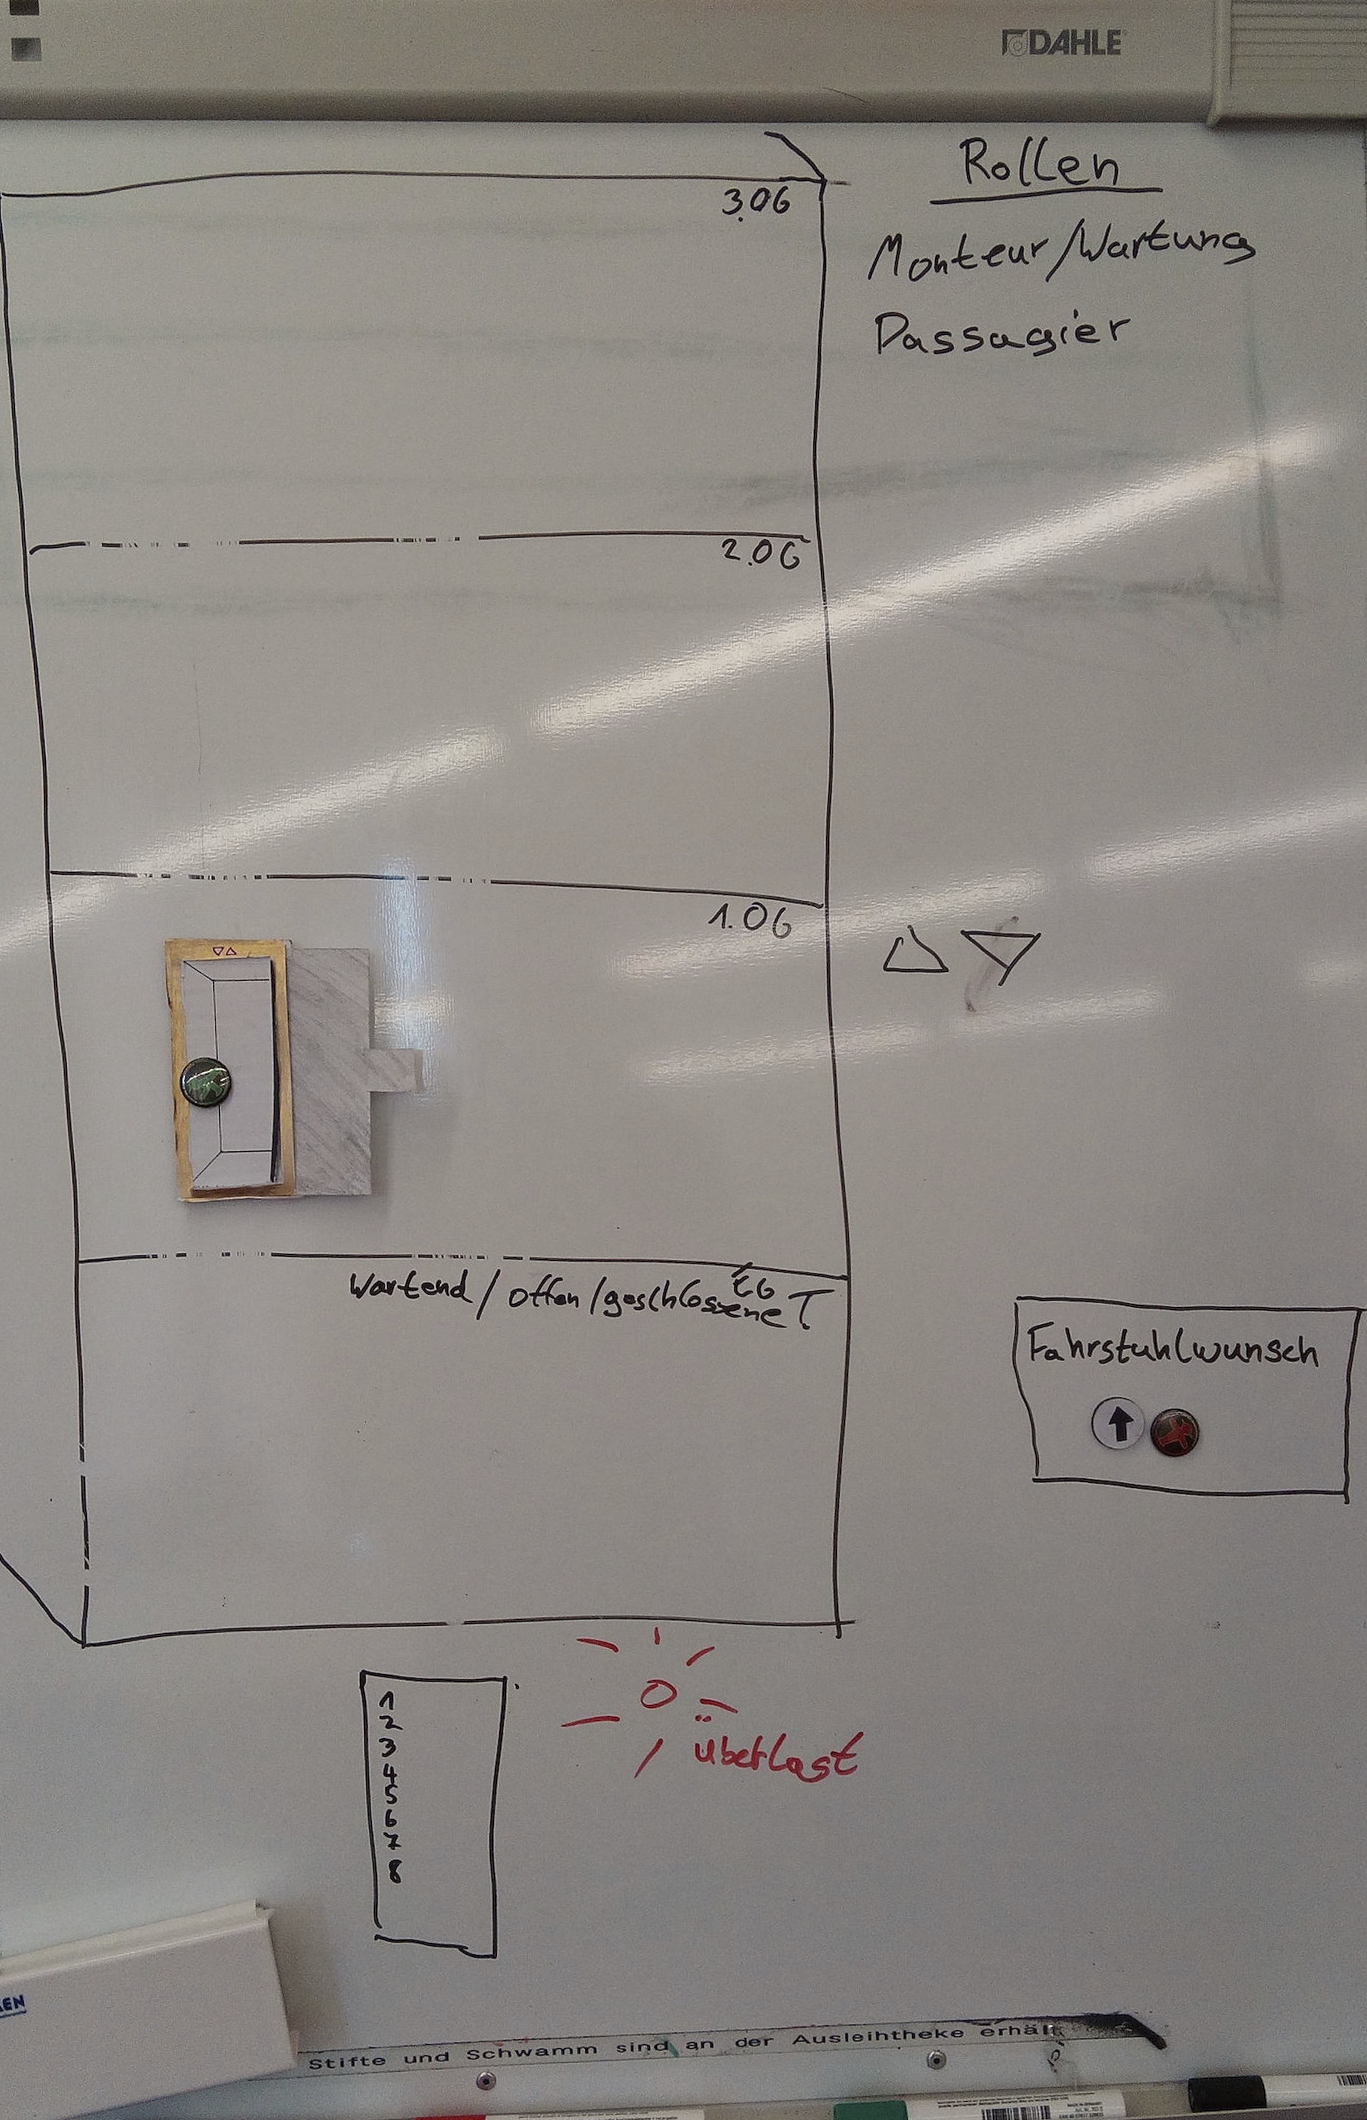
\includegraphics[height=8cm]{images/kundengespraech1.jpg}}
\subcaptionbox{Modell des Fahrstuhles}[0.49\linewidth]
{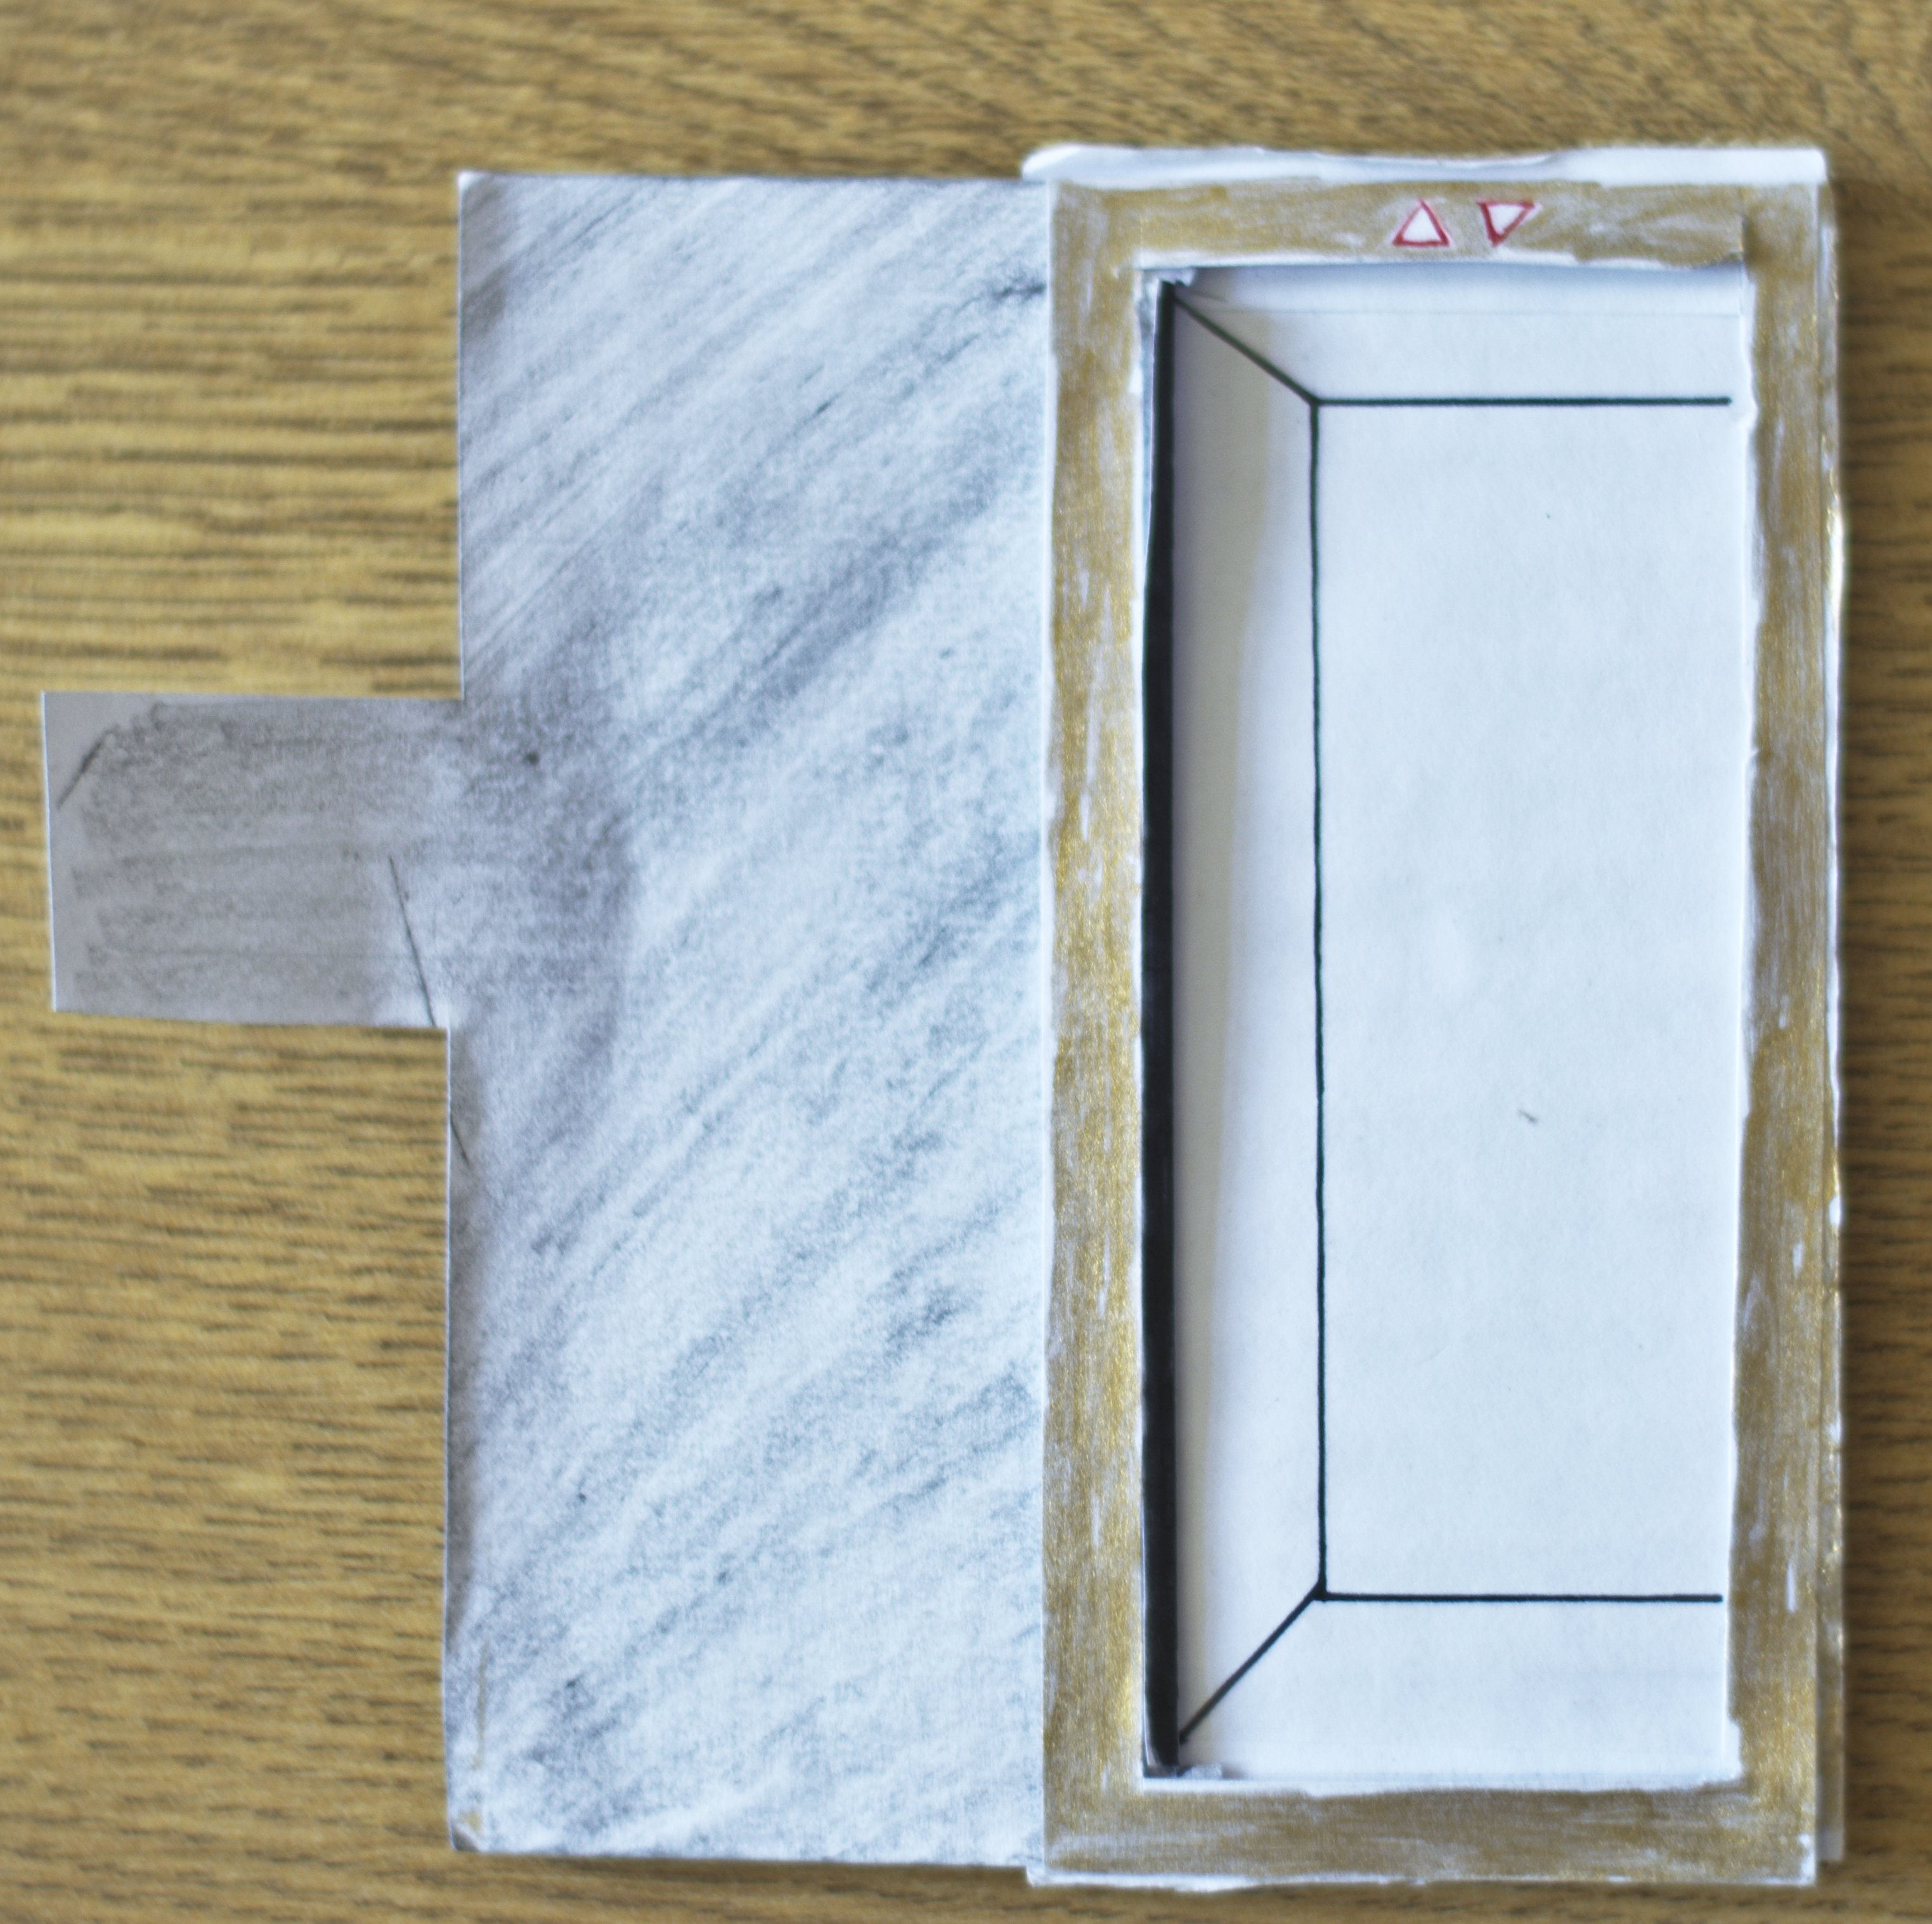
\includegraphics[height=8cm]{images/pappfahrstuhl.jpg}}
\caption{Kreativtechniken zur Anforderungsanalyse}
\end{figure}
Die folgenden grundlegende Fragen waren im Laufe der Analyse zu klären:
\begin{itemize}
	\item Wie viele Fahrstühle sollen verwendet werden können?
	\item Wie soll das Gebäude beschaffen sein?
	\item Welcher Algorithmus soll verwendet werden?
	\item Gibt es Schnittstellen zu anderen Systemen?
\end{itemize}
Weiterhin musste festgelegt werden ob die Priorität des Systems auf der Simulation oder auf einer möglichst realitätsnahen Umsetzung eines Liftes liegt. Im Laufe der Analyse und Modellierung entsprechender Anwendungsfälle wurde ersichtlich, dass das System sich aus zwei Teilsystemen, der \textbf{Fahrstuhlsteuerung} und der \textbf{Fahrstuhlsimulation} zusammensetzt, deren Anforderungen getrennt voneinander beschrieben werden mussten.\\
Eine Besonderheit des Systems ist dabei die Umgebung in der es eingesetzt werden soll, der Lehrbetrieb an einer Hochschule. Daraus ergaben sich spezielle Anforderungen, wie das Anzeigen der Zustandsübergänge, die gesondert betrachtet werden mussten.

\paragraph{}Vor allem aus den letztgenannten Anforderungen formte sich während der Analyse relativ früh unsere Vision einer Anwendung, welche in einer zweigeteilten Sicht Fahrstuhl und Zustandsdiagramm nebeneinander darstellt. Zusätzlich sollten Zustandsübergänge und aktive Zustände durch Animationen kenntlich gemacht werden.

\paragraph*{}Die Resultate der Analysephase, alle Anwendungsfälle und Vereinbarungen mit der Kundin wurden am Ende im Pflichtenheft festgehalten, welches als eigenständiges Dokument am Ende der Phase an die Kundin überreicht wurde. Diese Dokument war im weiteren Verlauf des Projektes ein zentrales Maß bei regelmäßigen Treffen und Evaluationen.



\chapter{Software-Entwurf}
Nach der Festlegung von Anforderungen und der Beschreibung der Funktionalitäten der Fahrstuhlsimulation war der nächste Schritt der Entwurf der internen Struktur. Wir näherten uns dieser Problemstellung von außen und erhöhten bei steigender Tiefe die Granularität. Dies bedeutete zunächst, die geeignetste Rahmen-Technologie festzulegen, welche die Anforderungen unseren Kundin am besten erfüllen konnte.

\section{Technologie}
Die Wahl der verwendeten Technologie fußte prinzipiell auf drei Hauptpunkten, erstens unserer Vision einer optisch ansprechenden Anwendung, welche das Zusammenspiel von System und dessen Zuständen visualisiert. Zweitens einer möglichst umfassenden Kompatibilität zu verschiedenen Plattformen und drittens der verfügbaren Zeit zur Realisierung aller Anforderungen. Wir entschlossen uns zunächst eine Vorauswahl zu treffen. Diese sollte wenn möglich Technologien enthalten, auf deren Gebieten bereits Erfahrungen im Team vorhanden waren. Nach kurzer Diskussion ergaben sich als Möglichkeiten die Nutzung von \textsc{C++}, \textsc{Java} oder \textsc{Web-Technologien} wie \textsc{Javascript}.

\paragraph*{}Nach reiflicher Überlegung und wiederholter Rücksprache mit unserer Kundin erschienen uns \textsc{Web-Technologien} am geeignetsten um alle Anforderungen in der zur Verfügung stehenden Zeit umzusetzen. Die Vorteile dieser Technologien, welche unsere Entscheidung maßgeblich beeinflussten, waren folgende:

\begin{enumerate}
	\item Sie ermöglichten uns größtmögliche Plattform-Kompa\-tibilität, da unser Produkt einerseits als Cross-Plattfom-Anwendung und andererseits als Web-Site veröffentlicht werden können.
	\item Mit den modernen Mitteln des Web-Designs war es uns möglich unsere Vision des Software-System umzusetzen.
\end{enumerate}

Gebündelt und verwendet wurden diese Möglichkeiten durch modere Werkzeuge der Web-Entwicklung wie beispielsweise \textsc{ReactJS}\footnote{\url{http://facebook.github.io/react/}}, \textsc{nodeJS}\footnote{\url{https://nodejs.org}}, \textsc{bower}\footnote{\url{http://bower.io}} oder \textsc{grunt}\footnote{\url{http://gruntjs.com}}. An dieser Stelle verweisen wir auf die entsprechenden Stellen der Entwicklerdokumentation.

\section{Algorithmus}
Bei der Wahl des zu implementierenden Fahrstuhl-Algorithmus lies uns die Kundin freie Hand. Im Kundengespräch wurde auch über die mögliche Erweiterung der Software um mehrere Algorithmen diskutiert. Dies hatte den Charme, dass Studierende damit zusätzlich die Möglichkeit gehabt hätten verschiedene Algorithmen zu vergleichen und zu erfahren wie stark oder weniger stark sich verschiedene Ansätze einer Problemlösung im Hinblick auf Algorithmus und Zustandsdiagramm unterscheiden. Letztlich wurde diese Erweiterung als \textit{mögliche Modifizierung} kategorisiert und ist nicht Teil dieses Projekts geworden.

\paragraph{}Wir entschieden uns im folgenden dazu einen Algorithmus zu verwenden, welcher in Fahrstuhlsystemen mit einem Schacht Anwendung findet, den \textit{Fahrstuhl-Algorithmus mit Sammelsteuerung}\cite{wiki_elev}. Hierbei fährt der Fahrstuhl zunächst in eine Richtung und bedient ausschließlich Fahrtwünsche oder -rufe die in dieser Fahrtrichtung existieren, andere werden gespeichert und nach Umkehr der Fahrtrichtung bedient.

\begin{figure}[h]
	\begin{minipage}{0.47\textwidth}
		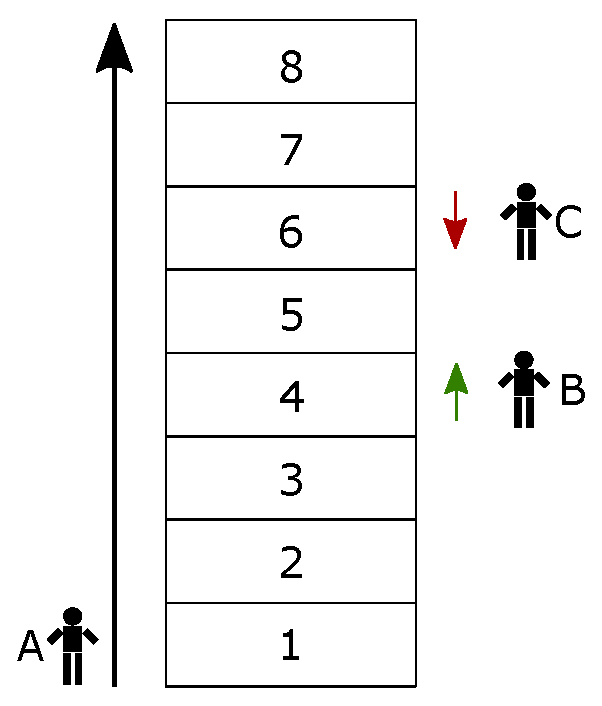
\includegraphics[width=\textwidth]{images/algo_example.eps}
		%\caption{Eine Grafik}
		%\label{Bild} 
	\end{minipage}
	% Auffüllen des Zwischenraums
	\hfill
	% minipage mit Grafik
	\begin{minipage}{0.47\textwidth}
		\paragraph{Beispiel}
		Passagier \textbf{A} steigt im Erdgeschoss zu und möchte in den achten Stock fahren. Während sich der Fahrstuhl in Bewegung setzt rufen ihn zwei weitere Personen auf Etage vier und sechs. Person \textbf{B} auf Etage vier ruft \textit{nach oben} und \textbf{C}, jene auf Etage sechs \textit{nach unten}.\\
		Während seiner Fahrt wird der Fahrstuhl nun den Ruf auf Etage vier bedienen, während er an Etage sechs vorbeifährt. Dieser Ruf wird im Anschluss nach Umkehr der Fahrtrichtung bedient.
		% \caption{Der Text}
		% \label{Text}
	\end{minipage}
	\caption{Beispiel zum Fahrstuhl-Algorithmus mit Sammel\-steuerung.}
	\label{algo_exam}
\end{figure}

\paragraph{}Wie man erkennen konnte setzt diese Form der Steuerung zwei Tasten je Etage zur Abgabe von Fahrtstuhlrufen voraus, weshalb diese in der vorliegenden Form implementiert wurden. Für weitere Informationen zu verschiedenen Fahrstuhl-Algorithmen verweisen wir auf folgenden Quellen \cite{wiki_elev} und \cite{wiki_elev_2}.

\newpage
\paragraph{Zustandsdiagramm}Nun galt es den Steuerungsalgorithmus näher zu analysieren, um ihn anschließend mittels \textsc{Javascript} zu implementieren. Dazu wurde über mehrere Gruppentreffen hinweg am Zustandsdiagramm des Systems gearbeitet. Abbildung \ref{ZD} zeigt das Resultat dieser Arbeit.

\begin{figure}[h]
	\hspace*{-2.0cm}
	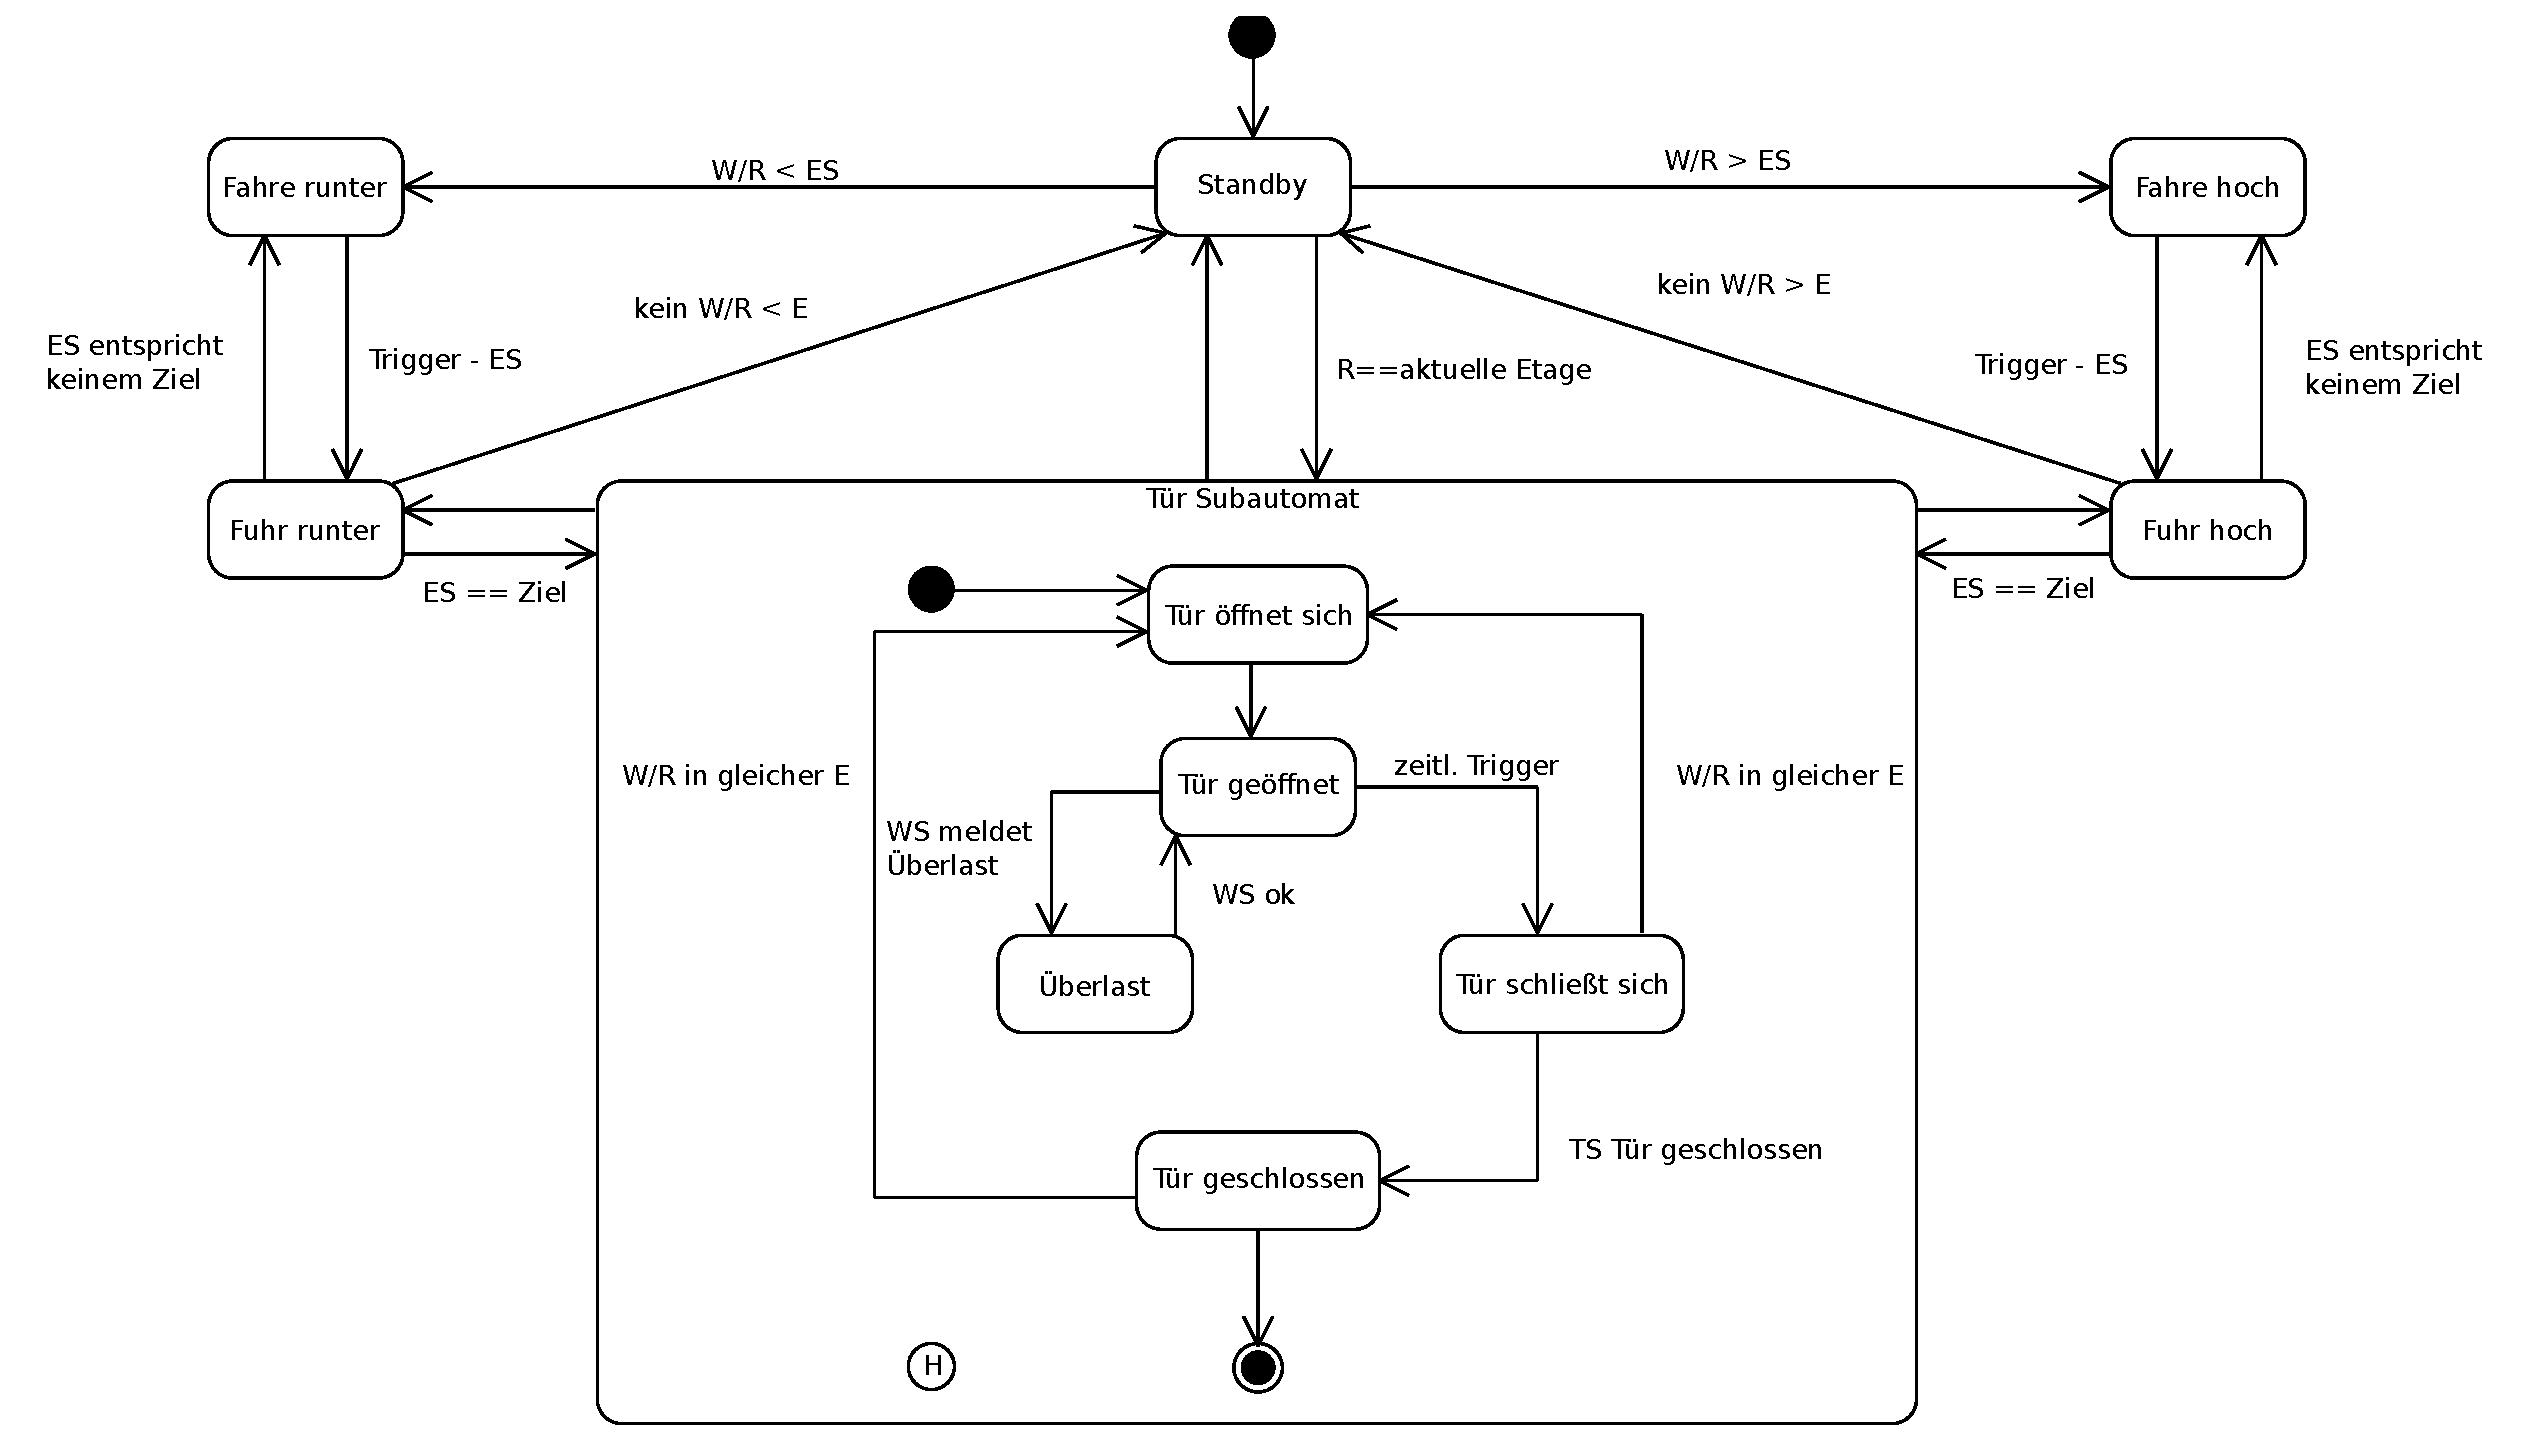
\includegraphics[width=1.3\textwidth]{images/ZDv6.eps}
	\caption{Zustandsdiagramm der Fahrstuhlsteuerung. Die im Diagramm verwendeten Abkürzungen erklären sich folgendermaßen: \textit{W}: Wunsch, \textit{R}: Ruf, \textit{ES}: Etagensensor, \textit{E}: Etage, \textit{WS}: WeightSensor oder Gewichtssensor, \textit{H}: History-Zustand}
	\label{ZD}
\end{figure}

\paragraph{Fahrt}
Den \textit{Standby}-Zustand nimmt die Steuerung in unserem System sowohl nach dem Start in Etage 1 als auch auf einer beliebigen Etage ein, sofern keine weiteren Wünsche oder Rufe vorhanden sind. Werden nun Rufe abgegeben, entscheidet die Steuerung auf Basis der Summe über und unter ihrer aktuellen Position, in welcher Richtung sie mit der Bearbeitung beginnt.

\paragraph{}Nehmen wir im Folgenden an, dass der Fahrstuhl nach oben fährt. In diesem Fall geht er zunächst in den Zustand \textit{Fahre hoch} über. Die Vorbeifahrt an einem Etagensensor \textit{ES} löst einen Übergang in den Zustand \textit{Fuhr hoch} aus, in welchem ein Mechanismus überprüft, ob die aktuelle Etage einem Wunsch/Ruf entspricht. Ist dies nicht der Fall, wird die Fahrt in der gleichen Richtung fortgesetzt, was dem erneuten Übergang in den Zustand \textit{Fahre hoch} entspricht.\\
Handelt es sich jedoch um eine Zieletage, geht die Steuerung in den \textit{Tür-Subautomat} über. Dieser entspricht einem sogenannten \textit{History-Zustand}\cite{history_Z}, welcher es uns elegant ermöglicht nach dem Verlassen des Subautomaten in einen Zustand gleicher Fahrtrichtung zurückzukehren.

\paragraph{Tür-Subautomat}
Mit dem Eintritt in den Subautomat öffnen sich zunächst die Fahrstuhltür. Im Zustand \textit{Tür geöffnet} können durch Betätigung des entsprechenden Buttons Fahrgäste hinzugefügt oder entfernt werden. Bei einer Anzahl von mehr als 8 Personen löst der Gewichtssensor \textit{ES} einen Übergang ein den Zustand \textit{Überlast} aus, welcher den Fahrstuhl am fahren hindert und nur durch das Entfernen von Passagieren verlassen werden kann.\\
Sollte die Weiterfahrt nicht durch Betätigung der Ruf- oder Wunschtaste der aktuellen Etage verhindert werden, geht der Fahrstuhl nach dem Schließen der Tür in den \textit{Fuhr hoch}-Zustand der letzten Fahrrichtung über.

\paragraph{}Nach der Abarbeitung aller Wünsche und Rufe geht die Steuerung in der aktuellen Etage des Fahrstuhls erneut in den \textit{Standby}-Zustand über. 

\section{Benutzerschnittstelle}
UI \todo{Wie haben wir uns das mit der UI gedacht und warum? Wie war der Weg dorthin?}

\section{Komponenten und Design Pattern}
Story? \todo{Wie leiten wir in unserem "from the outside to the inside" Approach am besten auf Architektur und Komponenten um?}

\paragraph{}Diese Vorauswahl bestand
Für die technische Umsetzung der Zustände in ausführbaren Quellcode ergaben sich folgende Entwurfsmuster:
\todo{Wir müssen aufpassen, dass wir eine klare Trennung zwischen Entwurfs-spezifischen Inhalten im Entwicklerhandbuch und hier vornehmen.}
\subsection*{State Design Pattern}
Vorteile, Nachteile, warum haben wir uns dageben entschieden?
\todo{Nachteile: großer Overhead, da hier nur 3 Zustände vorkommen, jedoch die Zustandsübergänge komplex sind}

\subsection*{Event Emitter}
\subsection{Observer Pattern}

\subsection*{Zustandstabelle}
\todo{nicht sinnvoll zwecks erweiterbarkeit/wartbarkeit}

Die eigentliche Herausforderung des Systems besteht nicht in den Zuständen, sondern in den Zustandsübergängen, da der Fahrstuhl bis auf wenige Ausnahmen wie von \textbf{Idle} nach \textbf{Stop} in jeden beliebigen Zustand springen kann.


\chapter{Qualitätssicherung}
\section{Allgemein}
Der Standard ISO/IEC 25000:2014 welcher als Einleitung zu genormten Methoden der Qualitätssicherung in der Software zu verstehen ist, definiert diese als "`Systems and Software Quality Requirements and Evaluation (SQuaRE)"'\cite[Foreword]{ISO25000}. Festzustellen ist: Der ISO25000 ist für einen Norm relativ jung ist und löst zwei Vorgänger, welche die Themen Softwarequalität bzw. Anforderungsanalyse (ISO/IEC 9126) und Software Evaluierung bzw. Test (ISO/IEC 14598) überwiegend getrennt behandeln ab. Neben der Motivation der Vermeidung von Redundanzen und Inkonsistenzen zwischen den zwei Normen, ist es Meinung des Autors, dass sich hierbei die Erkenntnis der notwendigen Verzahnung der beiden Teilgebiete zeigt. So werden z.B. im \textit{test driven development} idealerweise die Anforderungen direkt zur Software-Evulation benutzt.

\paragraph*{}Aus der Definition
\begin{quote}\label{PD_SQ}
software quality
capability of software product to satisfy stated and implied needs when used unter specified condidtions
\end{quote}\cite[4 Terms and definitions]{ISO25000}
lässt sich somit die umfassende Qualitätssicherung aufteilen auf
\begin{enumerate}
\item Einwirkung auf Anforderungsanalyse
\item Evaluation während und nach der Umsetzung
\end{enumerate}
da sich Softwarequalität nach obiger Definition rein auf die bereits eruierten Anforderungen und Bedingungen stützt, wie Gesamtzufriedenheit des Nutzers allerdings nur dann erreichen lässt, wenn diese Vorbetrachtung bestmöglich durchgeführt wurde.
\section{QS Anforderungsanalyse}
Zu Beginn des Projekts wurde beim der Erstellung des Pflichtenheftes auf vollständige und unmissverständliche Formulierungen geachtet, da Probleme in dieser Phase die größten Auswirkungen auf die Zufriedenheit des Nutzers besitzen.\\
Desweiteren wurde durch erneuten Vergleich der Anforderungen mit Kundenprotokollen und Aufgabenstellung sowie Prüfen auf Inkonsistenzen assistiert.

Als qualitätsunterstüzende Maßnahme wurden die Anforderungen möglichst auf sogenannte Issues, also Stichpunkte und Meilensteine in einem Projektmanager, abgebildet.
\section{QS Umsetzung}
\subsection{Allgemein}
\begin{itemize}
\item Konvetionen
\item Testregime
\end{itemize}
\subsection{Konventionen}
Bei der Mitarbeit von mehreren Personen an einem Projekt ergibt sich, durch unterschiedlichen Persönlichkeiten mit verschiedenen Heransgehensweisen und Vorerfahrung, schnell ein Zoo an Stilen und Gewohnheiten. Desweiteren besteht ein gewisser Konsensz, in der Branche, an bestimmen Herangehensweisen und Konvetionen ("`best practice"'). Daraus ergibt sich die Motivation feste Konventionen festzulegen, um entweder Bestehende zu vereinheitlichen oder sie für Jene, welche sie bis dato noch nicht kannten, einzuführen:
%Die Motivation dazu lasse ich hier bewusst herraus, diese möchte ich lieber im Vortrag dazu bennen. Gez. Markus 2015-06-24
\begin{itemize}
\item Allgemeine Konventionen
	\begin{itemize}
	\item Datum- und Zeitangaben in ISO 8601, Ausnahme bei nationalen externen Dokumenten möglich
	\item alle Daten sind zu Versionieren mit GIT, temporäre Datein jedoch nicht
	\item alle gefundenen Fehler in Issues/Gitlab festhalten
	\item Vektorgrafiken skaliert auf 100x100 px
	\item Textdatein in UTF8
	\end{itemize}
\item Konventionen Quelltext
	\begin{itemize}
	\item camelCase für Bezeichner
	\item keine nachgestellten Leerzeichen\footnote{engl. trailing whitespace}
	\item wenn möglich keine Zeile länger als 80 Zeichen %außer wenn's semantisch Sinn macht
	\item private Member mit einem Unterstrich
	\item Datei endet mit newline (leere Zeile)
	\item Javascript:
		\begin{itemize}
		\item ECMAScript 6
		\item "`use strict"' als erste Zeile eines .js
		\item Tabs statts Space
		\end{itemize}
	\end{itemize}
\end{itemize}


\subsection{Test}
Für die automatischen Tests wurde das Testframework Jasmine\footnote{http://jasmine.github.io}
\todo{Traceabillity hinzufügen -> jede Anforderung muss im Quellcode durch einen commit oder ähnlich nachverfolgbar sein}
\subsubsection{manuelle Testfälle}
\subsubsection{automatisierte Testfälle}

\chapter{Team-Organisation}
\section{Gruppenarbeit}
Um das Zusammenarbeiten in der Gruppe einfacher zu gestalten wurden verschiedene Technologien eingesetzt.
Zu finden von Terminen für Meetings wurde Doodle\footnote{\url{www.doodle.com}}  verwendet. Für die Kommunikation in der Gruppe Slack\footnote{\url{https://slack.com/}}.
\todo{Hier muss hin warum wir uns für JS und Co entschieden haben.}
\section{Verwendete Werkzeuge}
\section{Resümee}

\bibliographystyle{plaindin}
\bibliography{projektdokumentation}
